\begin{table*}[t]
\centering
\resizebox{\textwidth}{!}{
\begin{tabular}{lcccccccc}
\toprule
	\textbf{Model} & \textbf{GSM8K} & \textbf{MATH-500} & \textbf{AIME2024} & \textbf{AIME2025} & \textbf{AMC2023} & \textbf{OlympiadBench} & \textbf{AVG} \\
	\midrule
	Llama-3.1-8B-Instruct    & 75.89 & 35.20 & 4.17 & 1.04 & 23.59 & 12.00 & 25.32 \\
	\texttt{\ \ + 20K Gemini-Distill-Data}   & 54.89 & 22.60 & 1.04 & 0.63 & 12.03 & 7.41 & 16.43  \\
	\texttt{\ \ + 20K Claude4-Distill-Data}  & 63.76 & 35.80 & 1.04 & 0.83 & 23.44 & 13.48 & 23.06   \\
	\midrule
	Qwen-2.5-32B-Base        & 53.68 & 33.40 & 9.17 & 2.29 & 35.63 & 15.85 & 25.00  \\
	\texttt{\ \ + 20K Gemini-Distill-Data}   & 52.54 & 20.20 & 1.88 & 0.63 & 21.41 & 12.44 & 18.18  \\
	\texttt{\ \ + 20K Claude4-Distill-Data}  & 63.31 & 37.80 & 2.92 & 0.83 & 28.91 & 17.78 & 25.26  \\
	\midrule
	Qwen-2.5-32B-Instruct    & 93.71 & 81.00 & 15.60 & 14.17 & 69.84 & 42.22 & 52.76 \\
	\texttt{\ \ + 20K Gemini-Distill-Data}   & 63.68 & 32.80 & 15.00 & 2.92 & 35.63 & 19.11 & 28.19  \\
	\texttt{\ \ + 20K Claude4-Distill-Data}  & 76.88 & 54.80 & 17.71 & 13.96 & 55.00 & 30.96 & 41.55  \\
\bottomrule
\end{tabular}
}
\caption{Distillation Results from Gemini and Claude.}
\label{tab:distill}
\end{table*}
\begin{table*}[t]
\centering
\resizebox{\textwidth}{!}{
\begin{tabular}{lcccccccc}
\toprule
	\textbf{Model} & \textbf{GSM8K} & \textbf{MATH-500} & \textbf{AIME2024} & \textbf{AIME2025} & \textbf{AMC2023} & \textbf{OlympiadBench} & \textbf{AVG} \\
	\midrule
	Llama-3.1-8B-Instruct    & 75.89 & 35.20 & 4.17 & 1.04 & 23.59 & 12.00 & 25.32 \\
	\texttt{\ \ + 20K OSS-Summarized}   & 54.89 & 22.60 & 1.04 & 0.63 & 12.03 & 7.41 & 16.43  \\
	\texttt{\ \ + 20K QwQ-Summarized}  & 63.76 & 35.80 & 1.04 & 0.83 & 23.44 & 13.48 & 23.06\\
	\midrule
	Qwen-2.5-7B-Instruct & 83.24 & 74.00 & 12.50 & 7.08 & 22.66 & 38.07 & 39.59 \\
    \texttt{\ \ + 20K OSS-Summarized} & 82.34 & 72.60 & 12.50 & 6.46 & 21.41 & 27.70 & 37.17  \\
    \texttt{\ \ + 20K QwQ-Summarized} & 82.71 & 71.80 & 11.88 & 6.25 & 22.97 & 25.04 & 36.77  \\
	\bottomrule
\end{tabular}
}
\caption{Results from summarized Long CoT trajectories based on OpenAI-OSS and QwQ distilled trajectories.}
\label{tab:summarization}
\end{table*}

\begin{figure*}[t]
    \centering
    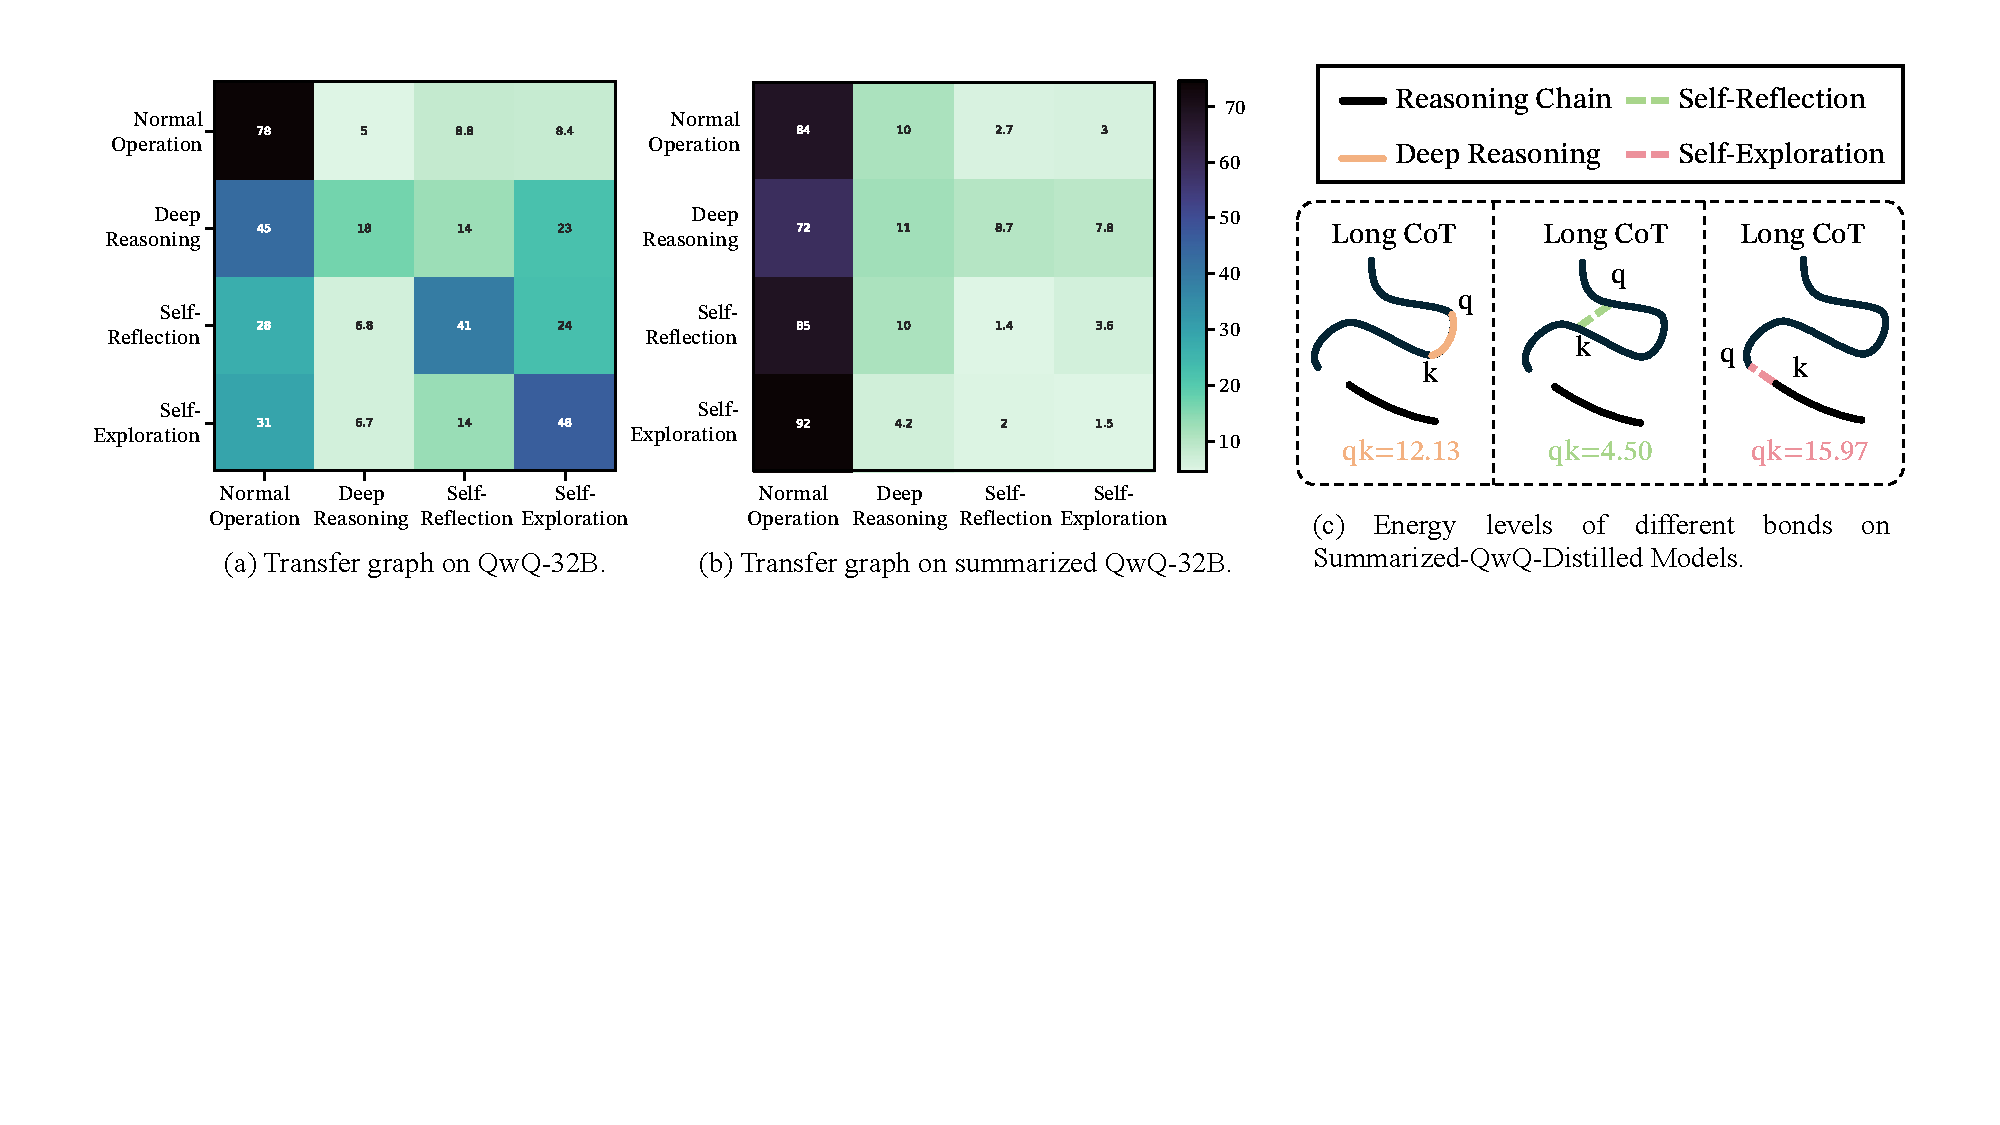
\includegraphics[width=0.98\textwidth]{figures/summary.pdf}
    \caption{The reasoning behavior distribution of summarized QwQ traces.}
    \label{fig:summary}
\end{figure*}

\section{Deteriorated Molecular Structure Cannot Be Easily Restored}

\paragraph{\textbf{How Current Private LLMs Protect Their Long CoT from Distillation?}}
Exposing reasoning traces allows LLMs to imitate both answers and procedures. 
Common defenses always consider compressing intermediate steps.
We quantify this by distilling from  Gemini-2.5-Pro-Thinking and Claude-4-Sonnet. Table~\ref{tab:distill} shows that beyond $\sim$45\% token reduction versus QwQ-32B rationales, distillation causes accuracy drops, showing compression can disrupt Long CoT structure.\vspace{-8pt}

\paragraph{\textbf{Summarization break reasoning bond distributions to prohibit distillation.}}
To further validate the effectiveness of summarization, we summarized Long-CoT traces from QwQ and R1. Table~\ref{tab:summarization} shows that training on compressed trajectories yields weaker performance than training on full traces and reduces distillation effectiveness by 2\%.
In Figure~\ref{fig:summary}, summarization shifts reasoning behavior distributions and creates a gap between observable outputs and internal error-bounded transitions, limiting trace inversion and behavioral cloning. However, compression can also protect model architecture and embedded inductive priors from unauthorized imitation.


\begin{TakeawayBox}{Takeaway 6}
Summarization and reasoning compression effectively protect Long CoT structures from distillation by disrupting structural coherence, preventing unauthorized replication of internal reasoning processes.
\end{TakeawayBox}